\documentclass{article}
\usepackage{graphicx}
\topmargin=0.0in
\oddsidemargin=0.0in
\evensidemargin=0in
\textwidth=6.5in
\marginparwidth=0.5in
\headheight=0pt
\headsep=0pt
\textheight=9.5in

\begin{document}
\begin{center}
	{
		\large{ANKUR PANWAR}
	}
\end{center}
\begin{flushleft}
D-5,New Defence Colony, \hspace{3.6in} Contact:9654471353\\
Bhopura, \hspace{3.5in} e-mailid: ankurrpanwar26@gmail.com\\
Ghaziabad-201005,\\
Uttar Pradesh\\
\end{flushleft}
\vspace{-0.3in}
\begin{figure}[h]
\hspace{4.4in}
	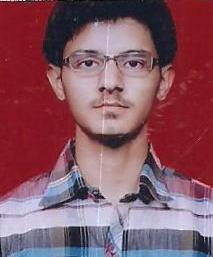
\includegraphics{img.jpg}
\end{figure}

\begin{flushleft}
	\textbf{OBJECTIVE}
	\vspace{-0.20in}
	\hspace{.5in}
	To work on SMART CITY projects
\end{flushleft}

\begin{flushleft}
	\vspace{0.30in}
	\textbf{EDUCATION}
	\hspace{0.45in}
	\begin{tabular}{|c|c|c|c|c|}
	\hline
	Degree&College/school&University/Board&Passing year&Pass Percentage\\
	\hline
	Senior Secondary&Kendriya Vidhyalya&CBSE&2014&91.3\\
	\hline
	B.Sc(H) Electronics&Maharaja Agrasen College&Delhi University&1st year&71%\\
	
	\end{tabular}
\end{flushleft}

\begin{flushleft}
	\vspace{0.30in}
	\textbf{PROJECTS}
	\begin{enumerate}
		\item Content syndication and catalogues for undergraduate science courses\\
		\item Non programed moving dustbin\\
		\item Advance Internal Combustion Engine( in progress)\\
		
	\end{enumerate}
\end{flushleft}

\begin{flushleft}
	\vspace{0.1in}
	\textbf{TRAINING AND INTERNSHIP}
	\begin{itemize}
		\item 3 month training in shree ram institute for webdesigning
	\end{itemize}
\end{flushleft}

\begin{flushleft}
	\vspace{.30in}
	\textbf{RESEARCH \\PUBLICATION}
	\begin{enumerate}
		\item Presented poster on ELECTROMAGNETIC WAVES AND ITS SUSTAINANCE. Publication International Journal for Scientific Research andDevelopment
	\end{enumerate}
\end{flushleft}

\begin{flushleft}
	\vspace{0.2in}
	\textbf{TECHNICAL SKILLS}
	\begin{itemize}
		\item Programing language(c,c++,embedded c)
		\item Markup languages(HTML,CSS)
		\item Autocad,photoshop,corel draw,multisim
		\item Typing speed 35 wpm
		\item Proficient in circuit designing
	\end{itemize}
\end{flushleft}

\begin{flushleft}
	\vspace{0.30in}
	\textbf{SOFT SKILL}
	\begin{enumerate}
		\item self motivational skills
		\item communication skills
		\item leadership 
		\item team-working skills
		\item time management and ability to work under pressure
	\end{enumerate}
\end{flushleft}

\begin{flushleft}
	\vspace{0.2in}
	
		\textbf{EXTRA CURRICULAR ACTIVITIES}
	\begin{itemize}
		\item Attending workshops
	 	\item Member of Student council
	\end{itemize}
\end{flushleft}

\begin{flushleft}
	\vspace{0.2in}
	
		\textbf{CO-CURRICULAR ACTIVITIES}
	\begin{enumerate}
		\item swimming
	 	\item singing
		\item playing football
	\end{enumerate}
\end{flushleft}

\begin{flushleft}
	\vspace{0.4in}
	\textbf{Personal Details}\\
	\hspace{1.5in}Mother's name:\hspace{.08in}ANITA PANWAR\\
	\hspace{1.5in}Father's name:\hspace{.1in}RAVINDER PANWAR\\
	\hspace{1.5in}Sex:\hspace{.75in}Male\\
	\hspace{1.5in}Date of birth:\hspace{.15in}26th October 1995\\
	\hspace{1.5in}Nationality:\hspace{.27in}Indian\\
	\hspace{1.5in}Marital status:\hspace{.09in}Unmarried\\
\end{flushleft}
\begin{flushleft}
	\vspace{0.1in}
	\textbf{Reference}\hspace{0.36in}: Dr. Praveen Kant Pandey (M.sc, Ph.D), Contact details: +919910158848\\
\end{flushleft}
\end{document}